\subsection{Pruebas de concepto: \texttt{OpticalFlow} y \texttt{YOLO}}

El desarrollo del módulo de procesado del video afectaba al tratamiento de datos que se iba a realizar posteriormente, por esto mismo se decidió 
tratarlo como el primer problema a solucionar.

Dentro de este módulo se busca automatizar la obtención de datos y parametrización del movimiento de las truchas dentro del video.

En este sentido se plantearon dos alternativas para su desarrollo usando diferentes tecnologías:

\begin{enumerate}
    \item \textbf{Solución basada en \textit{OpticalFlow}}: La idea general de este método es caracterizar el movimiento de la trucha respecto al 
    fondo de la imagen.\newline
    Si tenemos en cuenta que el análisis por \texttt{OpticalFlow} nos da como resultado una serie de vectores que representan el cambio en los 
    píxeles de la imagen, cabe la posibilidad de obtener una serie de vectores globales que represen el movimiento de los bordes de la trucha entre fotogramas. 
    La representación de esta idea se puede ver en la \autoref{fig:IdeaOF}.

    \begin{figure}[H]
        \centering
            \begin{subfigure}[b]{\textwidth}
                \centering
                \begin{subfigure}[b]{0.25\textwidth}
                    \centering
                    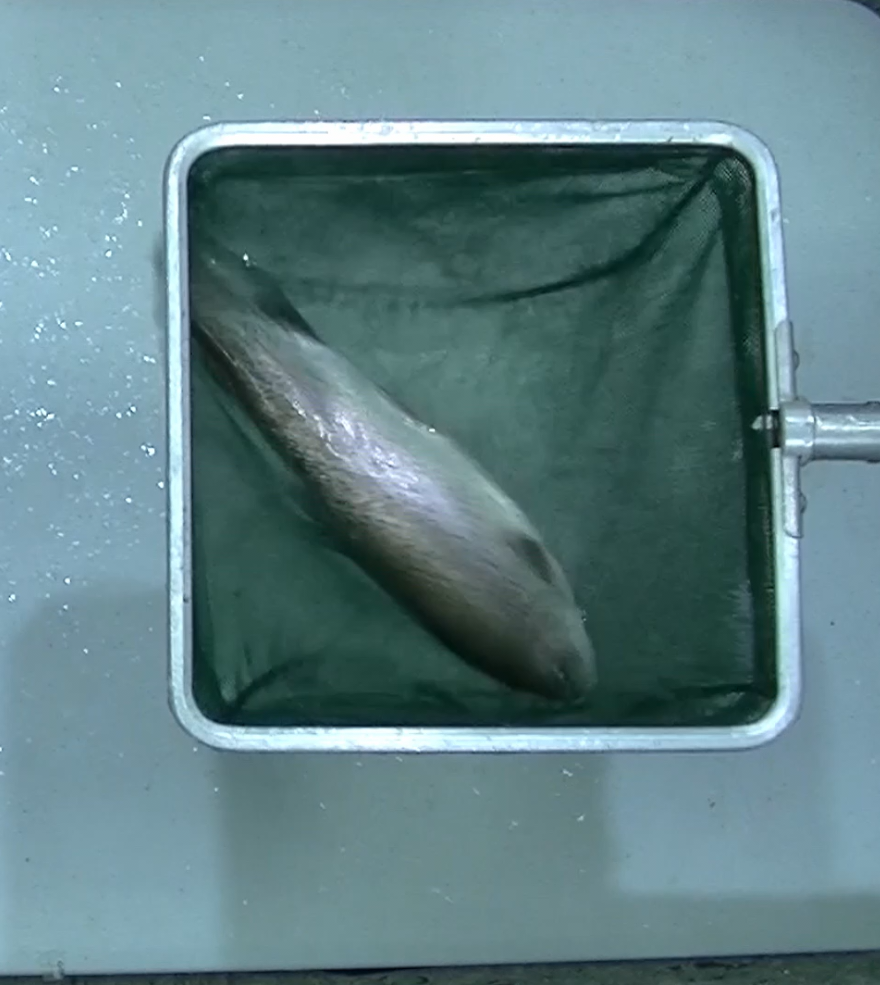
\includegraphics[width=0.8\textwidth]{images/6/SinOptical2.png}
                    \label{fig:SinOptical2}
                \end{subfigure}
                \begin{subfigure}[b]{0.25\textwidth}
                    \centering
                    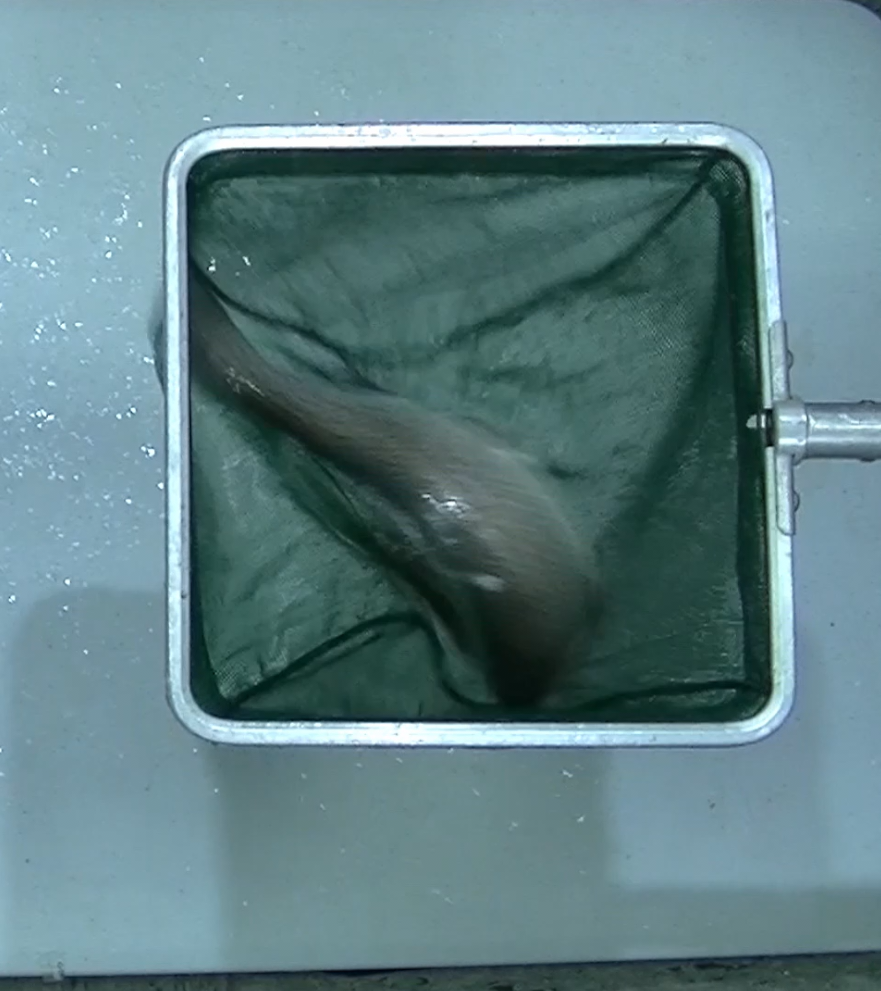
\includegraphics[width=0.8\textwidth]{images/6/SinOptical3.png}
                    \label{fig:SinOptical3}
                \end{subfigure}
                \begin{subfigure}[b]{0.25\textwidth}
                    \centering
                    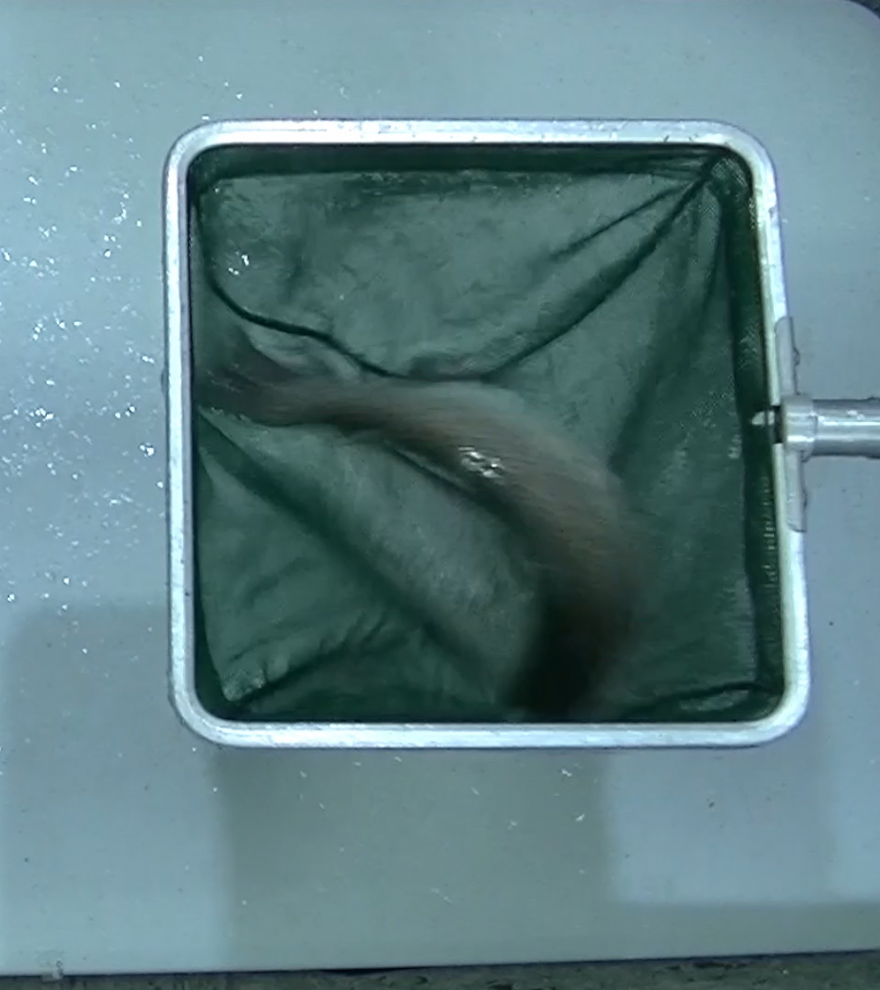
\includegraphics[width=0.78\textwidth]{images/6/SinOptical4.png}
                    \label{fig:SinOptical4}
                \end{subfigure}
                \caption{Fotogramas de entrada}
                \label{fig:FotogramasEntrada}
            \end{subfigure}
            \begin{subfigure}[b]{\textwidth}
                \centering
                \begin{subfigure}[b]{0.25\textwidth}
                    \centering
                    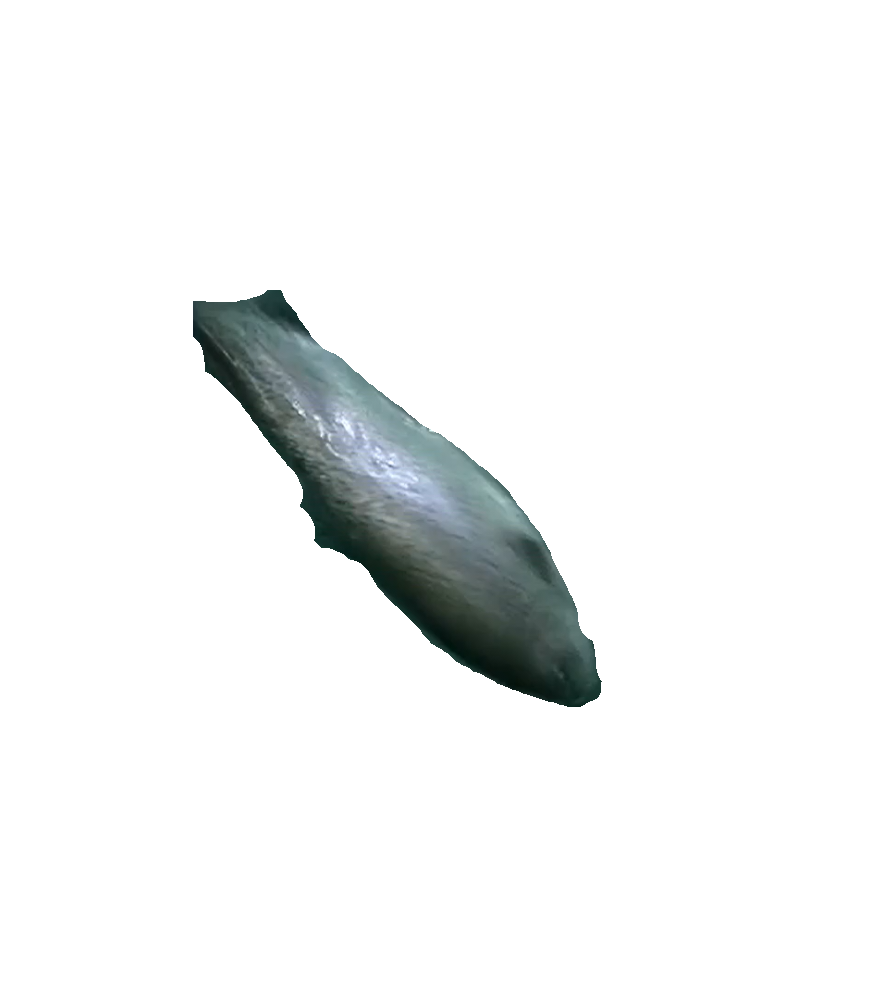
\includegraphics[width=0.8\textwidth]{images/6/Vacio2.png}
                    \label{fig:Vacio2}
                \end{subfigure}
                \begin{subfigure}[b]{0.25\textwidth}
                    \centering
                    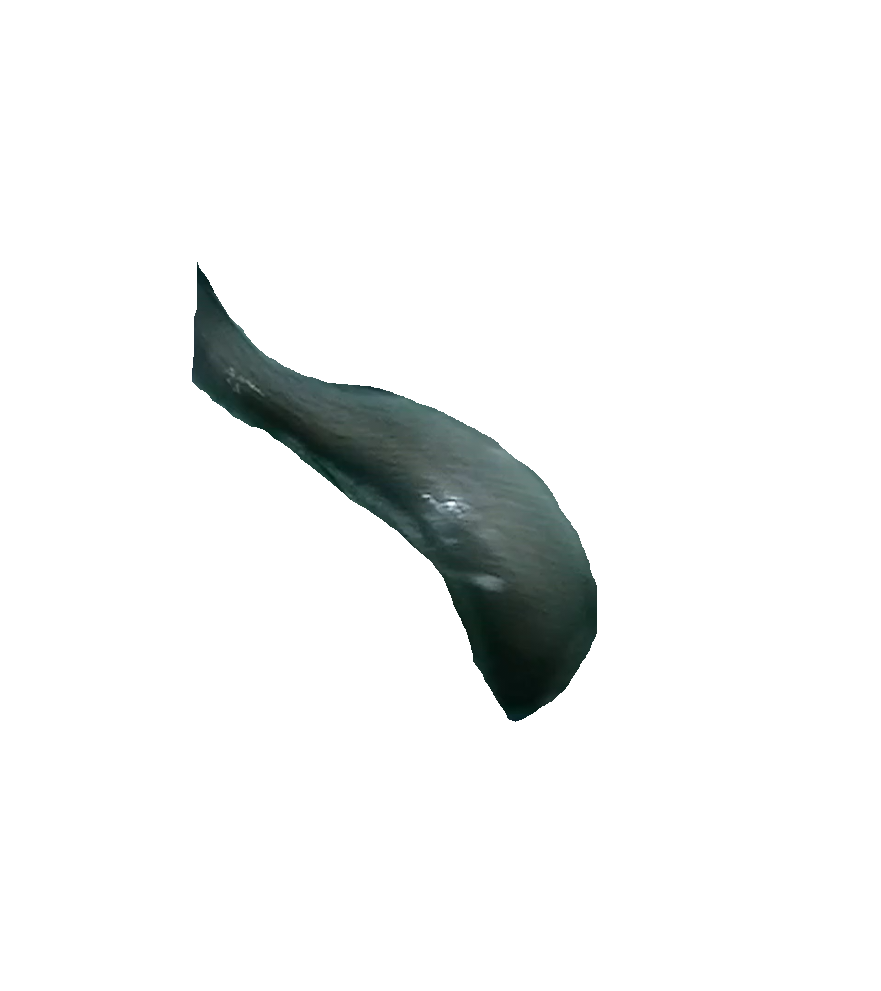
\includegraphics[width=0.8\textwidth]{images/6/Vacio3.png}
                    \label{fig:Vacio3}
                \end{subfigure}
                \begin{subfigure}[b]{0.25\textwidth}
                    \centering
                    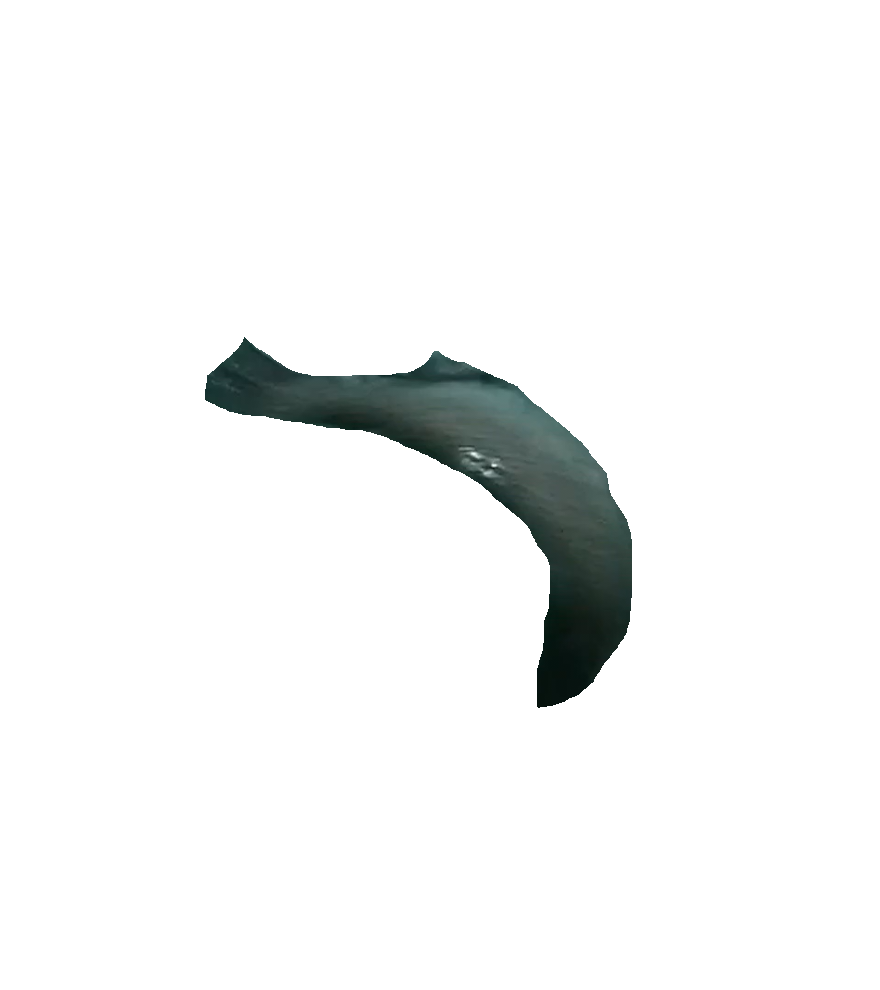
\includegraphics[width=0.8\textwidth]{images/6/Vacio4.png}
                    \label{fig:Vacio4}
                \end{subfigure}
                \caption{Fotogramas con el fondo eliminado}
                \label{fig:FotogramasSilueta}
            \end{subfigure}
            \begin{subfigure}[b]{\textwidth}
                \centering
                \begin{subfigure}[b]{0.25\textwidth}
                    \centering
                    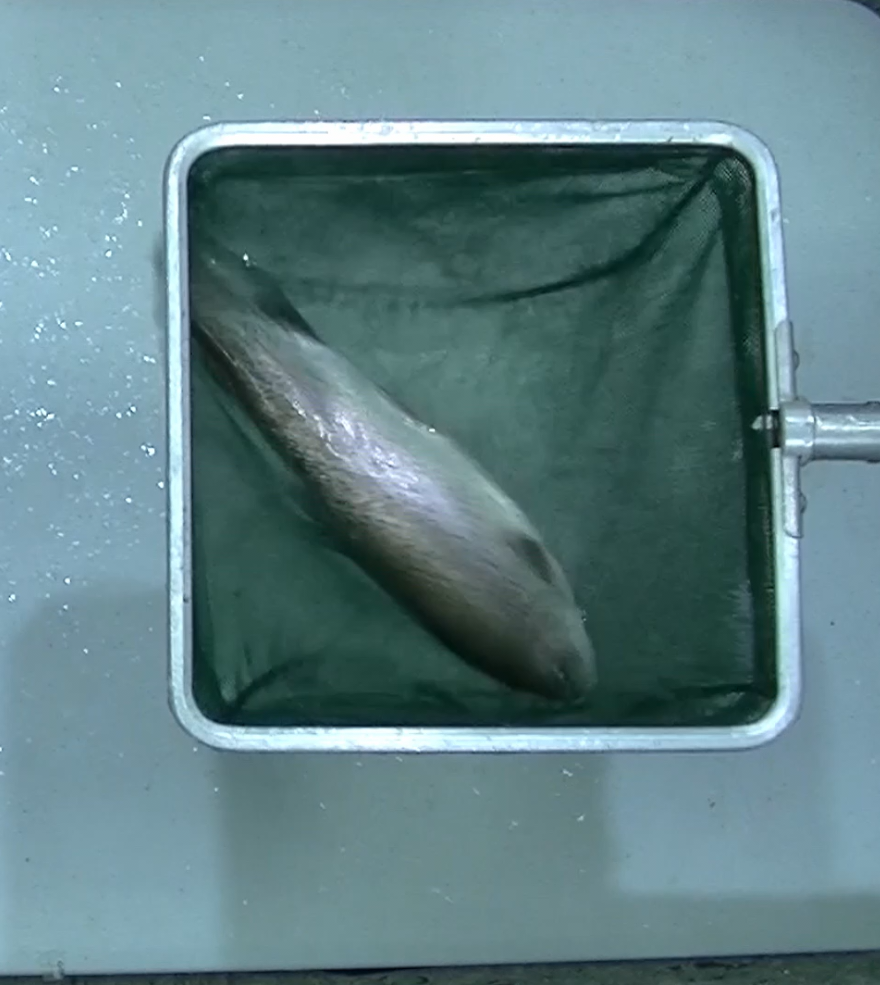
\includegraphics[width=0.8\textwidth]{images/6/SinOptical2.png}
                    \label{fig:Opt2}
                \end{subfigure}
                \begin{subfigure}[b]{0.25\textwidth}
                    \centering
                    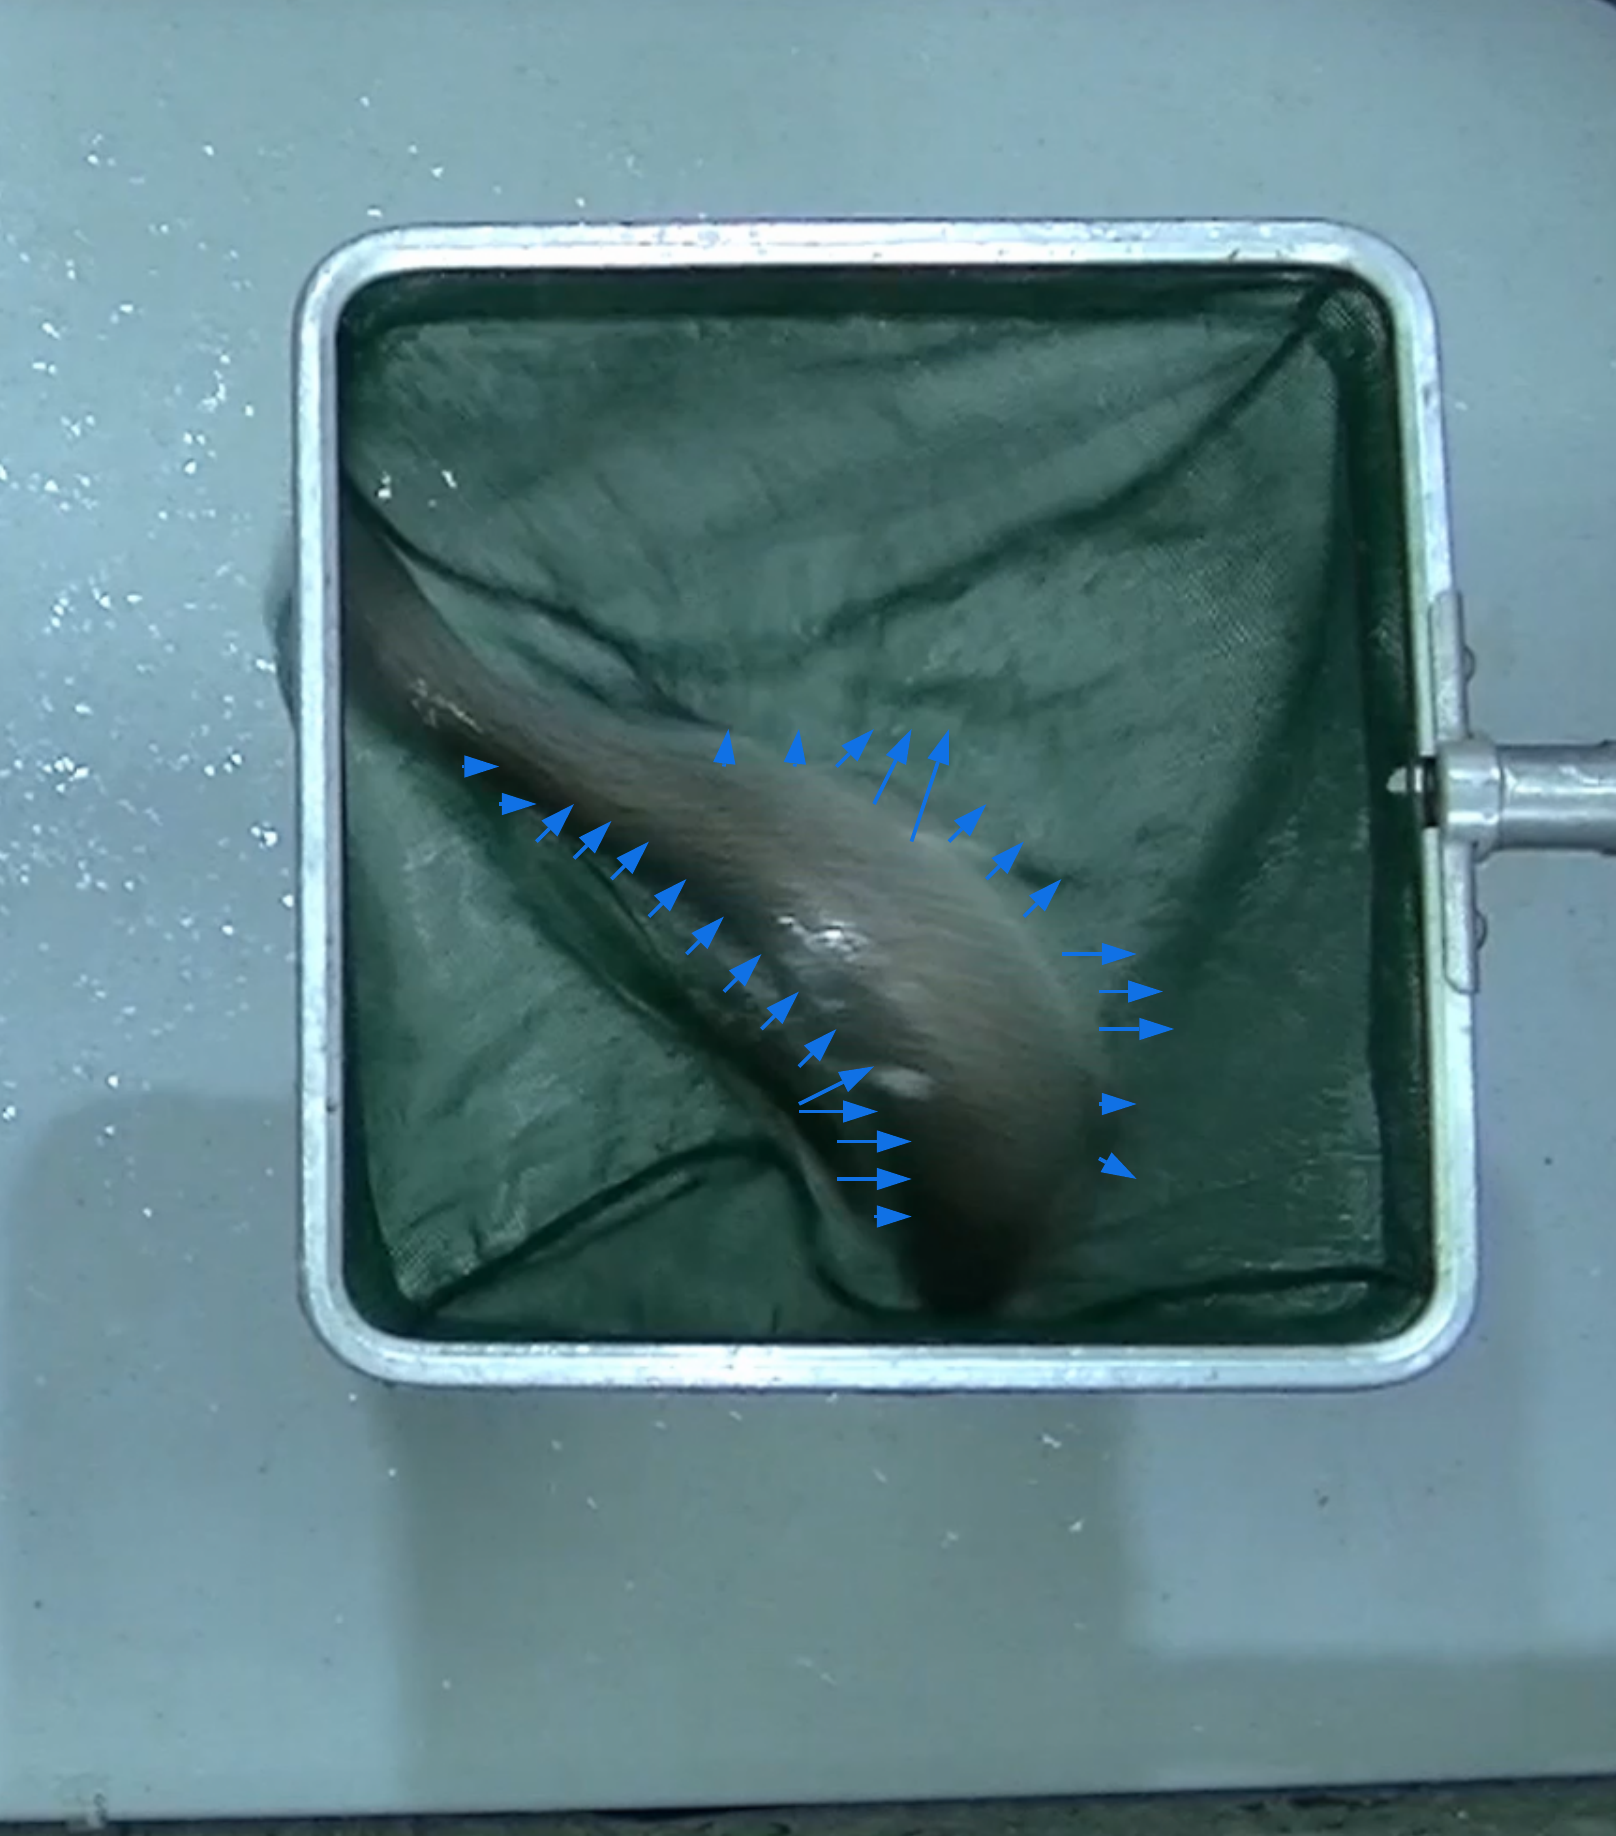
\includegraphics[width=0.8\textwidth]{images/6/ConOptical3.png}
                    \label{fig:Opt3}
                \end{subfigure}
                \begin{subfigure}[b]{0.25\textwidth}
                    \centering
                    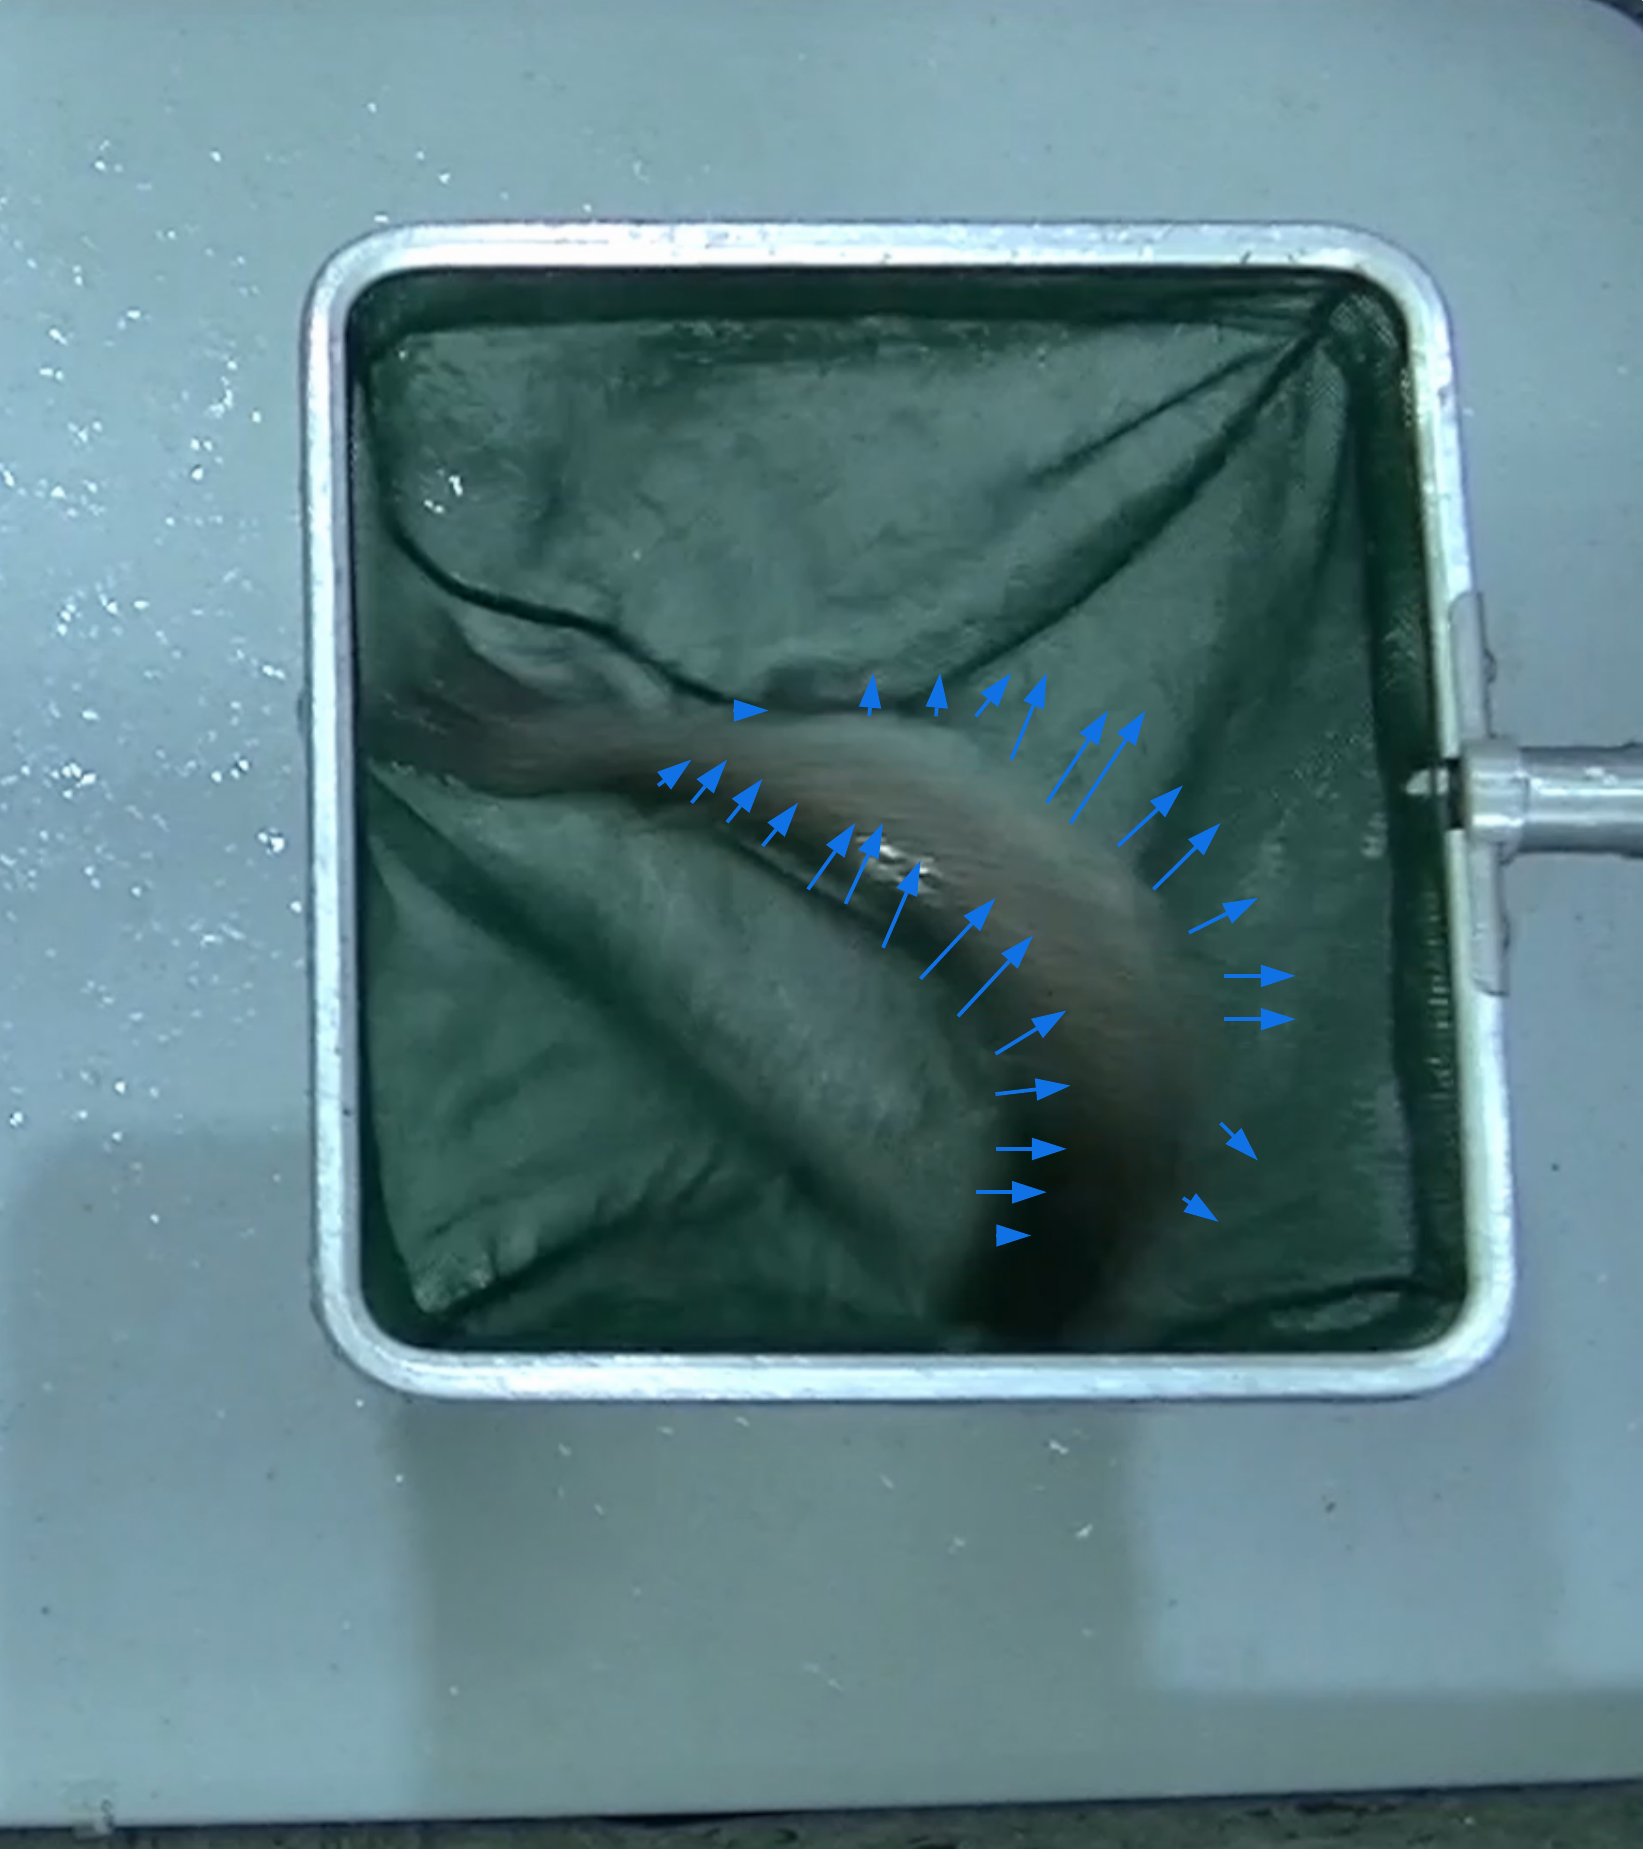
\includegraphics[width=0.8\textwidth]{images/6/ConOptical4.png}
                    \label{fig:Opt4}
                \end{subfigure}
                \caption{Representación de los vectores que se buscan obtener}
                \label{fig:FotogramasSalidaOF}
            \end{subfigure}
    \caption{Idea general basada en \texttt{OpticalFlow} para el módulo de procesamiento del video}
    \label{fig:IdeaOF}
    \end{figure}

    Como se puede observar, la idea es obtener un conjunto de vectores en el contorno del pez que nos permitan 
    saber diferentes datos:
    \begin{itemize}
        \item Si se ha movido o no: a través de la suma de todos los vectores y la obtención del 
        módulo del vector global. Si este valor es mayor que cierto umbral, se podría indicar que está sucediendo 
        un movimiento entre los dos fotogramas.
        \item Hacia donde se ha movido: a través del análisis de la dirección del vector global se puede indicar 
        el sentido del movimiento que está ocurriendo.
    \end{itemize}

    \item \textbf{Solución basada en el uso de \textit{YOLO} como herramienta de análisis}: A través del uso de una \texttt{\acrshort{cnn}} 
    se procesa el video, obteniendo información sobre los objetos detectados como truchas.\newline
    Para realizar esto, hay que definir la tarea que realizaría la red:
    \begin{itemize}
        \item Clasificación: no es útil, ya que no aporta información sobre la posición de los objetos detectados en la imagen.
        \item Segmentación: puede ser útil, pero para entrenar la red en esta tarea, los datos etiquetados deben ser segmentos de la imagen. 
        Esto puede llevar demasiado tiempo y; como se verá más tarde, no es la única tarea que puede aportar información para la automatización.
        \item Detección: es la más interesante, ya que nos permite conseguir unos tiempos de procesado por imagen muy bajos a la vez que nos da datos 
        relacionados con la posición y el tamaño aproximado de una caja rectangular que envuelve al pez.
    \end{itemize}
    
    Teniendo en cuenta lo anterior, lo más viable es entrenar un modelo \texttt{YOLO} en tarea de detección de truchas. Esto es realizable a través de la creación 
    de un conjunto de datos de imágenes de truchas y sus respectivas etiquetas, que en este caso son dos esquinas de la caja (\texttt{Bounding Box}) que engloba el 
    objeto que se quiere detectar.\newline
    La red neuronal entrenada podra ser capaz de devolver datos sobre las truchas detectadas y las posiciones y tamaños de las cajas que las engloban.
    
    A través de estas \texttt{Bounding Boxes}, podemos parametrizar un movimiento como la reducción del área o movimientos de la posición de la \texttt{Bounding Boxes}.

    \begin{figure}[H]
        \centering
        \begin{subfigure}[t]{0.39\textwidth}
            \centering
            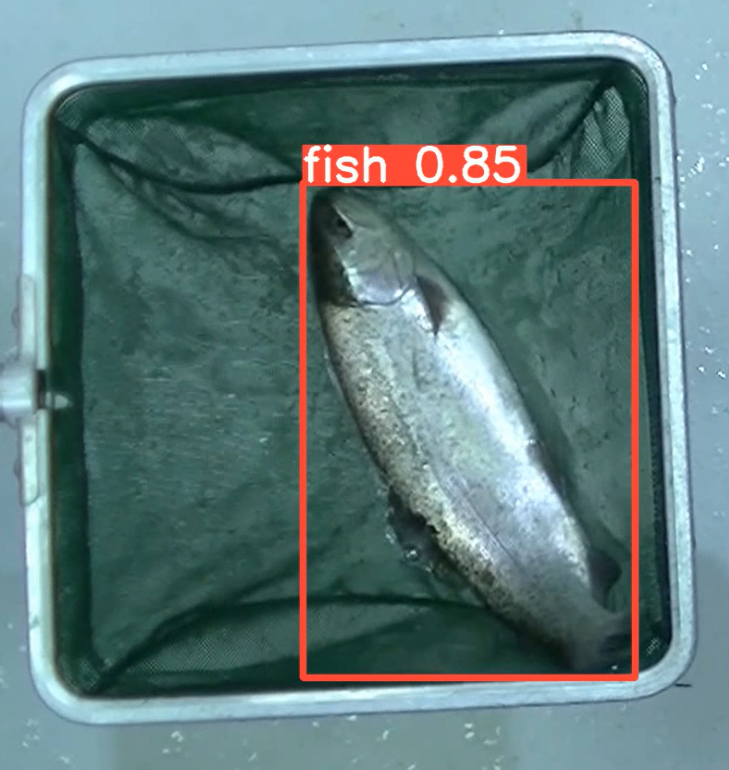
\includegraphics[width=0.8\textwidth]{images/6/EjemploYOLO.png}
            \caption{Imagen procesada por \texttt{YOLO}}
        \end{subfigure}
        \begin{subfigure}[t]{0.59\textwidth}
            \centering
            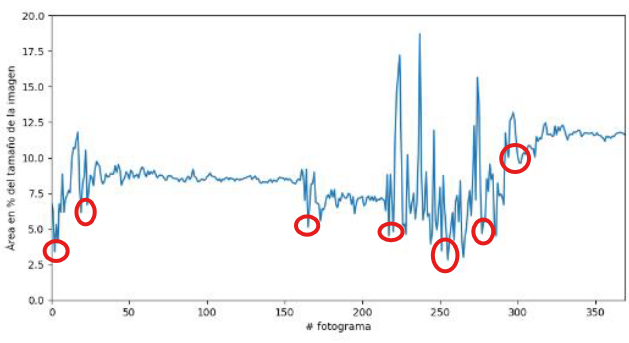
\includegraphics[width=0.99\textwidth]{images/6/YOLOEjemploResultados.png}
            \caption{Idea de estimación de movimiento a través de los resultados de las \texttt{Bounging Boxes}, marcando en rojo los movimientos}
        \end{subfigure}
        \caption{Idea general basada en \texttt{YOLO} para el módulo de procesamiento del video}
        \label{fig:IdeaYOLOGeneral}
    \end{figure}

    Hay que tener en cuenta que sería necesario hacer una validación de los entrenamientos realizados para conseguir cumplir con las necesidades. 
    Esto es debido a que, al contrario que el \texttt{OpticalFlow}, las redes neuronales no son deterministas y dependiendo del fotograma sobre el que se realice inferencia, 
    podemos obtener resultados alejados de los esperados.
\end{enumerate}

\vspace{1\baselineskip}
Para decidir qué método podía dar mejores resultados, se probaron las diferentes tecnologías aplicadas en el video \verb|23_NT_R1_J1_P7_8.mp4|. Este video dura 15 segundos y contiene dos peces, uno a 
la izquierda y otro a la derecha.

\clearpage
\subsubsection{Pruebas de concepto con \texttt{OpticalFlow}}

Para realizar las pruebas se utilizó el entorno de \texttt{MATLAB} en la versión \texttt{2023B}. En esta aplicación se disponen de 2 funciones principales 
que implementan análisis de flujo óptico: 
\begin{itemize}
    \item Método de Horn-Schunck: método de análisis denso (aplicado para todos los píxeles de la imagen).
    \item Método de Lucas-Kanade: método de análisis local (aplicado a áreas de píxeles que se asumen que tienen el mismo movimiento).
\end{itemize}

Ambas pruebas demostraron que los videos con los que se estaba trabajando tenían una tasa de fotogramas demasiado baja para la cantidad de movimiento que podía ocurrir entre fotogramas. 
Esto se puede observar en el flujo óptico percibido cuando suceden cambios bruscos del pez como en la \autoref{fig:HSOpticalFlow} para el método Horn-Schunck y en la \autoref{fig:LKOpticalFlow} 
para el método Lucas-Kanade.

\begin{figure}[H]
    \centering
    \begin{subfigure}[b]{0.49\textwidth}
        \centering
        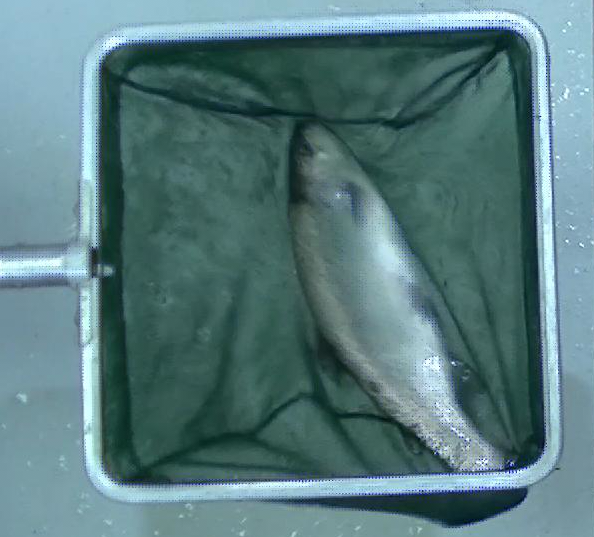
\includegraphics[width=0.95\textwidth]{images/6/6.2.1/HSIzquierda1.png}
    \end{subfigure}
    \begin{subfigure}[b]{0.49\textwidth}
        \centering
        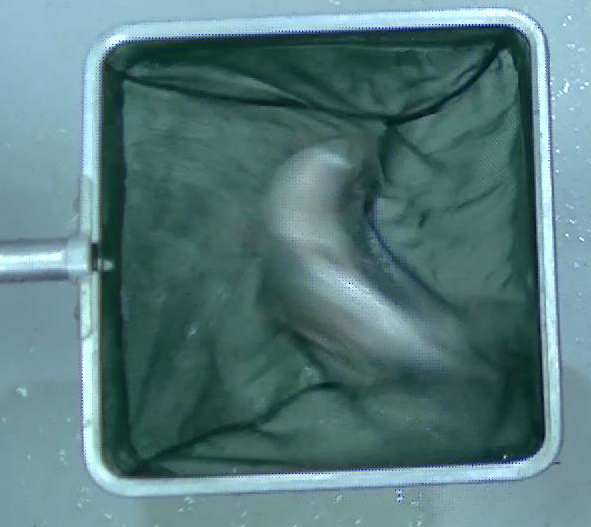
\includegraphics[width=0.95\textwidth]{images/6/6.2.1/HSIzquierda2.png}
    \end{subfigure}
    \caption{Flujo óptico detectado entre dos fotogramas por el método Horn-Schunck en los videos del \textit{NetText}}
    \label{fig:HSOpticalFlow}
\end{figure}

\begin{figure}[H]
    \centering
    \begin{subfigure}[b]{0.45\textwidth}
        \centering
        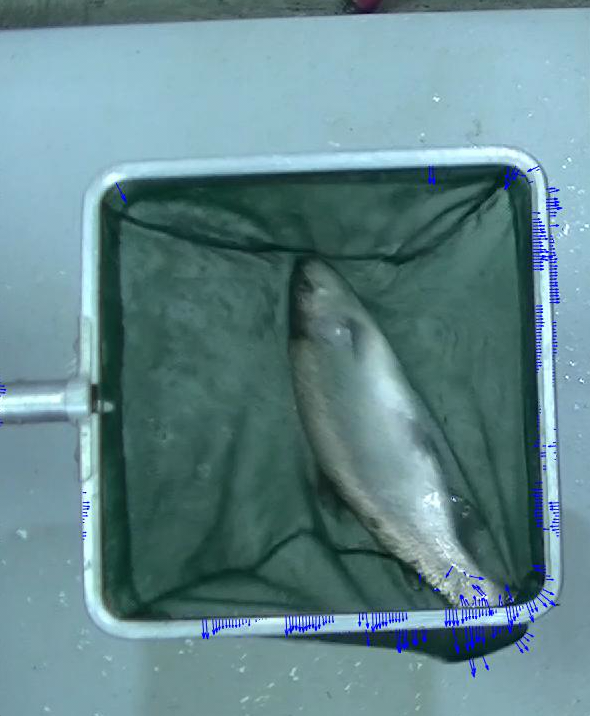
\includegraphics[width=0.8\textwidth]{images/6/6.2.1/LKIzquierda1.png}
    \end{subfigure}
    \begin{subfigure}[b]{0.45\textwidth}
        \centering
        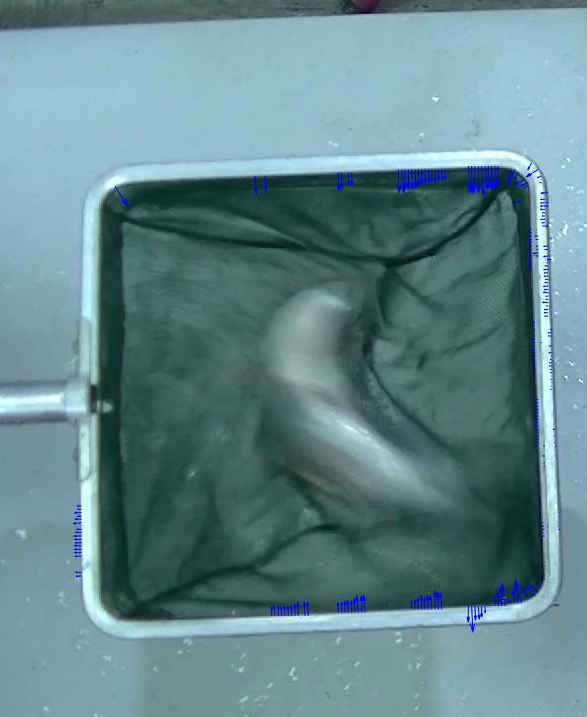
\includegraphics[width=0.8\textwidth]{images/6/6.2.1/LKIzquierda2.png}
    \end{subfigure}
    \caption{Flujo óptico detectado entre dos fotogramas por el método Lucas-Kanade en los videos del \textit{NetText}}
    \label{fig:LKOpticalFlow}
\end{figure}

El principal problema del método Horn-Schunck es que se ve muy afectado por el ruido, en el caso de este experimento, ese ruido aparece por la poca \texttt{tasa de fotogramas} y la falta de \texttt{bitrate} 
que tiene el video en comparación con la velocidad de movimiento que tienen las truchas. Aparte de esto, es un método computacionalmente muy costoso. En el caso de este video de 15 segundos tardó cerca de 10 
minutos en realizar el análisis completo del flujo óptico, lo cual incumple el requisito 18.

Vemos cierta mejoría usando el método de Lucas-Kanade, pero al realizar el análisis de forma local en zonas con similitudes, en cuanto la trucha hace un movimiento, el análisis deja de funcionar 
sobre la parte de la imagen en la que se sitúa la trucha. Aún siendo bastante rápido (sin llegar a ser tiempo real), esta situación elimina la posibilidad de utilizar este método para la 
parametrización del movimiento de la trucha.

En ambos métodos se ha comprobado que mejorarían los resultados aplicando umbralizaciones a la imagen. También sería necesario un preprocesado para delimitar la sección de 
imagen sobre la que es de interés realizar el análisis de flujo óptico (la zona de la red que contiene la trucha). Aún con lo comentado anteriormente, el único método que puede aportar algún 
tipo de información de manera consistente para todo el video es el método de Horn-Schunck.

\subsubsection{Pruebas de concepto con \texttt{YOLO}}

Para realizar esta prueba, creo un conjunto de datos con el que entrenar a través de fotogramas del video \verb|23_NT_R1_J1_P1_2.mp4|. Esto se realizó a través de la herramienta \texttt{\acrfullr{cvat}}.\newline
Esta herramienta de código abierto\cite{cvat.aicorporationComputerVisionAnnotation2023} es mantenida por los creadores de la librería \texttt{OpenCV}. Dispone de una versión online limitada al número de 
archivos que se pueden subir a \texttt{500 MB} y en otros aspectos, pero también dispone de una versión desplegable por \texttt{Docker}. Uno de sus puntos fuertes y el motivo de su uso en este trabajo es 
la compatibilidad con muchos formatos de exportación de etiquetas.

Como parte de este proyecto y como sistema que sirviese de soporte para guardar todos los conjuntos de datos necesarios, se desplegó como contenedor en el servidor \acrfullr{nas} del \acrfullr{gamma}.

Con esta aplicación se realizó el etiquetado de 24 imágenes para realizar un primer entrenamiento, el conjunto de datos se dividió de la siguiente manera:
\begin{itemize}
    \item 16 imágenes para el conjunto de entrenamiento.
    \item 4 imágenes para el conjunto de validación.
    \item 4 imágenes para el conjunto de pruebas.
\end{itemize}

Posteriormente se realizó el entrenamiento de la red neuronal \texttt{YOLOv8} versión \texttt{nano}, que es la más pequeña y rápida de entrenar. Los detalles en profundidad de resultados de este 
entrenamiento se pueden observar en el \hyperref[train:1]{anexo B}. \newline
Se consiguió unos buenos resultados y al inferir sobre el video \verb|23_NT_R1_J1_P7_8.mp4|, se observó que el seguimiento de la trucha se conseguía incluso en situaciones críticas donde la trucha realizaba 
el movimiento como en la \autoref{fig:YOLOTrain1Bien}. Sin embargo, situaciones como las de la \autoref{fig:YOLOTrain1Mal},en donde la trucha tenía formas suficientemente extrañas o se ocultaba detrás del marco de la red resaltaron la falta de entrenamiento y la 
necesidad de expandir el conjunto de datos.
\begin{figure}[H]
    \centering
    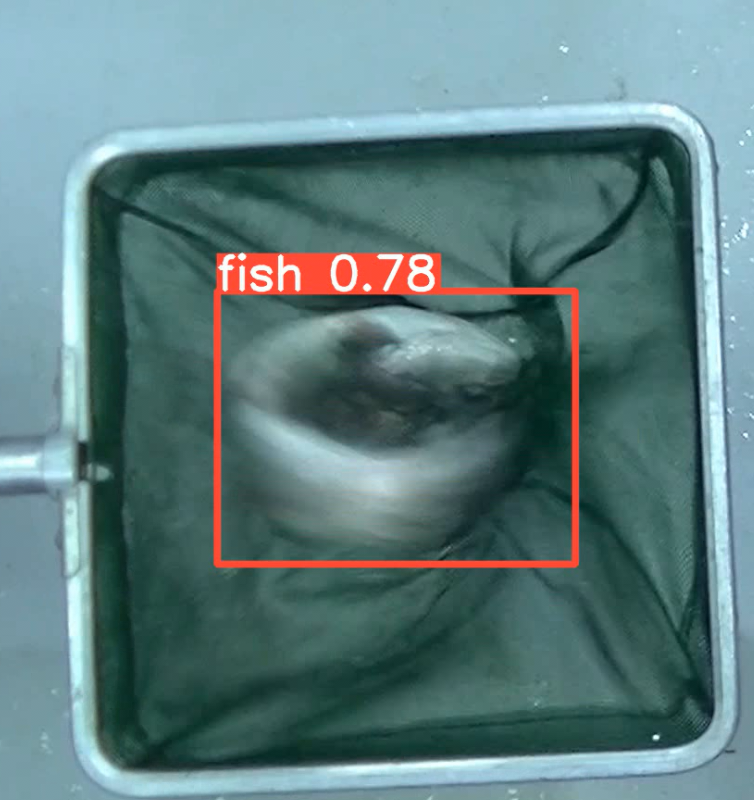
\includegraphics[width=0.31\textwidth]{images/6/6.2.2/DeteccionTrain1.png}
    \caption{Correcta detección en la prueba de concepto de \texttt{YOLO} en situaciones de movimiento}
    \label{fig:YOLOTrain1Bien}
\end{figure}

\begin{figure}[H]
    \centering
    \begin{subfigure}[b]{0.4\textwidth}
        \centering
        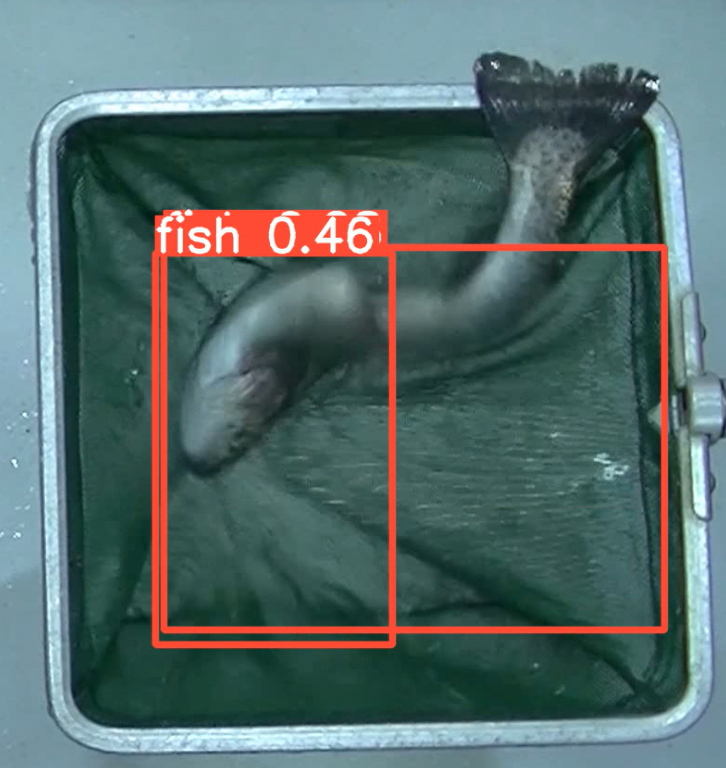
\includegraphics[width=0.7\textwidth]{images/6/6.2.2/DeteccionRaraTrain1.png}
        \caption{Detección de poca confianza y de baja calidad en el primer entrenamiento}
    \end{subfigure}
    \begin{subfigure}[b]{0.5\textwidth}
        \centering
        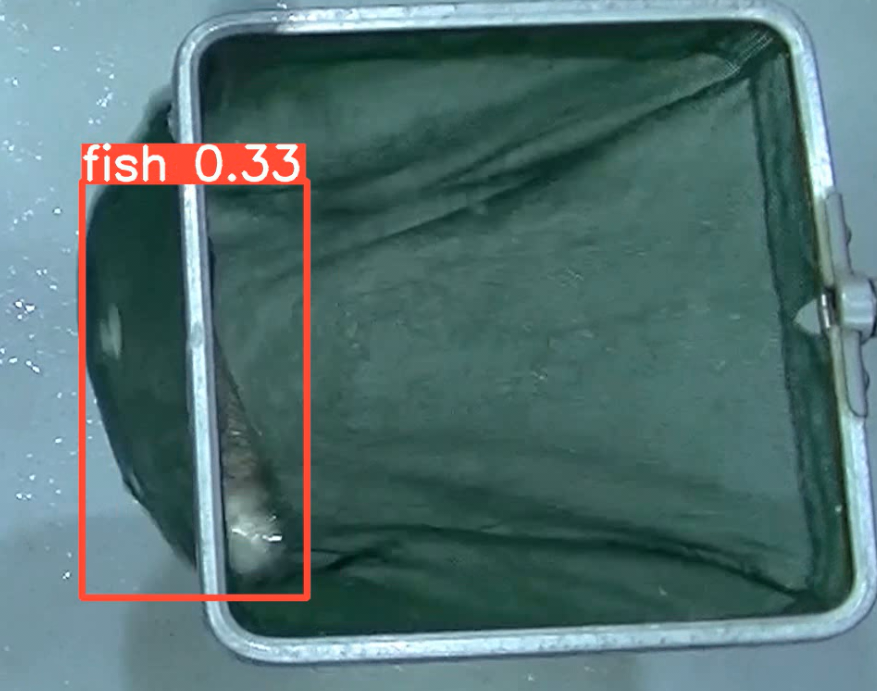
\includegraphics[width=0.7\textwidth]{images/6/6.2.2/PocaConfianzaTrain1.png}
        \caption{Detección de poca confianza por ocultación de la trucha}
    \end{subfigure}
    \caption{Situaciones negativas en la prueba de concepto de \texttt{YOLO}}
    \label{fig:YOLOTrain1Mal}
\end{figure}

Aún con los problemas varios que se pudieron observar, se observó que en una \texttt{\acrshort{gpu}} \texttt{GTX 1060 6GB} de \texttt{NVidia} el procesado del video y la obtención de los resultados solo tardaba \texttt{10 ms} 
por fotograma de video. Esto permitiría un procesado menor al tiempo del video hasta con 100 \acrshort{fps}.

Esta prueba de concepto demuestra la viabilidad del uso de \texttt{YOLO} como herramienta para obtener datos sobre las truchas existentes en el video de forma rápida.

Teniendo en cuenta que la mayoría de los movimientos observables de las truchas se basan en coletazos, podemos determinar que la trucha cuando busca realizar un movimiento, tendrá que comprimir su cuerpo en un menor 
área y después volver a estirar el cuerpo. Esto es directamente caracterizable con los datos de las \texttt{Bounding Boxes} obtenidos usando \texttt{YOLO}.

\vspace{2\baselineskip}

\subsubsection{Análisis de las pruebas de concepto}

En los anteriores puntos se presentaron dos alternativas:
\begin{itemize}
    \item \textbf{OpticalFlow}: aunque es una solución que idealmente debería funcionar, es incapaz de tener la suficiente consistencia con los videos usados en este trabajo, que tienen demasiado movimiento entre fotogramas. Aparte 
    de esto, un punto negativo severo es que el único algoritmo que consigue sacar algo de información vectorial sobre el flujo en las zonas del pez es de tipo denso, tardando una relación de 40 veces la duración del video en procesar 
    el resultado. Esto incumple el requisito de acelerar el experimento para los investigadores del \textit{NetTest}.
    \item \textbf{YOLO}: aún con situaciones con problemas de detección, pueden ser en mayor grado solucionado con mayor entrenamiento y expansión del conjunto de datos. Como la tarea que realiza son solo de detección, alcanza unas 
    velocidades que permiten la viabilidad del proyecto.
\end{itemize}

Por lo anterior, se ha decidido finalmente descartar la solución basada en \texttt{OpticalFlow} y utilizar un modelo \texttt{YOLO} como base para el análisis y obtención de datos del video. 

Gracias a estas pruebas de concepto, se realizaron unas gráficas representativas sobre el cambio de área y centroide para demostrar la viabilidad de contar movimientos con este sistema. Esto se utilizó para el 
aporte en un artículo de conferencia sobre el mismo tema llevado a cabo por el investigador Álvaro de la LLave-Propín\cite{delallave-propinEstilosAfrontamientoHacia2024}.

\clearpage
\subsection{Entrenamiento progresivo de los diferentes modelos de \texttt{YOLO}}

En la librería de \texttt{ultralytics}, existen dos modelos de detección que se busca soportar en el desarrollo de esta solución para el procesado de los videos:

\begin{itemize}
    \item Detección tradicional con \texttt{Bounding Boxes} con ejes paralelos a los ejes de la imagen.
    \item Detección con \acrfullr{obb}, que es capaz de minimizar el área que define al pez, pero tarda más en realizar el procesamiento y tiene resultados en distinto formato.
\end{itemize}

Habitualmente, la detección tradicional, al no tener que lidiar con rotación, es capaz de ser mucho más rápida en el tiempo de inferencia, pero la posibilidad de desarrollar el sistema soportando redes de tipo \texttt{OBB} 
puede permitir manejar mejores precisiones en un futuro.

Al usar la herramienta de etiquetado \texttt{CVAT} se observó que la exportación a etiquetas para un modelo \texttt{YOLO OBB} no eran funcionales. Estas etiquetas requieren para cada imagen un archivo \texttt{.txt} que contenga 
todas las instancias de los objetos en la imagen y los cuatro puntos que definen el cuadro que lo delimita.\newline
Para poder entrenar la red \texttt{OBB}, se usó una herramienta disponible en un repositorio de \texttt{GitHub}\cite{kolesnikovKoldim2001COCO_to_YOLOv82024} que transformaba etiquetas en formato \texttt{COCO} (formato estándar 
que se estructura en un \texttt{XML}) a las etiquetas necesarias. 

En este proyecto, se busca obtener buenos resultados en el entrenamiento para ciertos estadísticos, siendo el más importante la precisión de la \texttt{Bounding Box}, ya que queremos que se ajuste lo máximo posible al mínimo tamaño 
necesario. También nos interesa mucho las métricas de precisión y obtener un área máxima bajo la curva \texttt{F1}, ya que tiene en cuenta la precisión y, si conseguimos buenos resultados en la parte alta para la confianza, implicará 
que tenemos un buen número de verdaderos positivos respecto a falsos positivos con buena precisión. Al trabajar con una sola clase, los estadísticos relacionados con el ámbito de clasificación no son tan relevantes siendo que se 
cumpla un mínimo de clasificación en las detecciones.

Lo primero que se realizó fue un pequeño aumento de datos. Como se buscaba que la red generalizase mejor el concepto de trucha, se añadieron imágenes sin truchas como las de 
la \autoref{fig:VaciasTrain2}, en la que apareciesen la mesa vacía y partes de la red vacías.

\begin{figure}[H]
    \centering
    \begin{subfigure}[t]{0.55\textwidth}
        \centering
        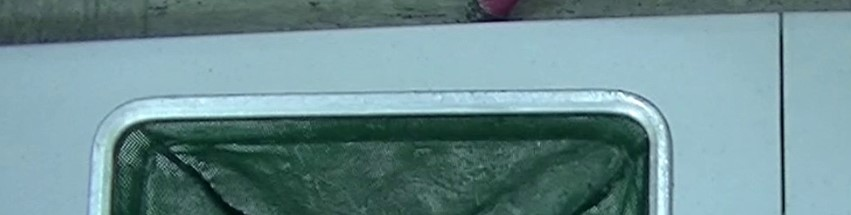
\includegraphics[width=0.9\textwidth]{images/6/6.3/esquinaTopVacia.jpg}
        \caption{Imagen de esquina vacía del segundo conjunto}
    \end{subfigure}
    \begin{subfigure}[t]{0.4\textwidth}
        \centering
        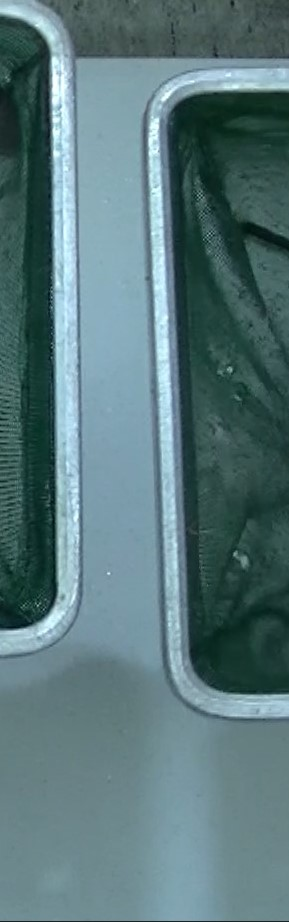
\includegraphics[width=0.3\textwidth]{images/6/6.3/medioVacio.jpg}
        \caption{Imagen del área entre las truchas añadida al segundo conjunto}
    \end{subfigure}
    \caption{Imágenes extra para el segundo conjunto sin truchas}
    \label{fig:VaciasTrain2}
\end{figure}

Esto permitió al modelo entrenado tener mejor capacidad de generalización de las truchas, además de tener menos falsos positivos (ver \hyperref[train:2]{anexo B: entrenamiento 2}). En otro entrenamiento 
posterior aumentando las épocas hasta 300, se observó que se podía seguir reduciendo el error asociado al ajustado de las \texttt{Bounding Boxes} (ver \hyperref[train:3]{anexo B: entrenamiento 3}), por lo 
tanto para los siguientes entrenamientos se decidió trabajar con un número de épocas mayor o igual a 300.
\clearpage

Posteriormente, se decidió usar el conjunto de videos antiguos del \textit{NetTest} para expandir el conjunto de datos. Esto se debía a 3 razones principales:
\begin{enumerate}
    \item \textbf{Aumento de datos y creación de un modelo más robusto}: el usar imágenes como las de los videos antiguos permitiría una capacidad alta al modelo de detectar truchas bajo diferentes condiciones de luz y de diferentes tamaños (las de esos videos son 
    jóvenes). Además de esto, los movimientos de los peces en los videos antiguos eran más difíciles de analizar por su falta de detalle, mejorando la cantidad de datos que representaban movimiento.
    \item \textbf{Evitar Overfitting para futuros entrenamientos}: el \texttt{overfitting} es una situación conocida en el entrenamiento de redes neuronales en las que las redes son entrenadas de forma excesiva, aprendiendo el ruido
     del conjunto de datos. Esto se ve representado por la incapacidad del modelo de predecir correctamente sobre datos que no haya visto en ningún momento del entrenamiento. No es una situación que deba suceder, pero cuanto más 
    variado sea el conjunto de datos, menos posibilidades hay de llegar a esta situación.
\end{enumerate}

En total se añadieron 34 imágenes de los videos antiguos, dando como resultado un conjunto de datos de 84 imágenes que se dividieron en subconjuntos entrenamiento, validación y prueba con la relación 70-15-15.\newline
Con este conjunto de datos se realizaron 2 entrenamientos(ver \hyperref[train:4]{anexo B}), uno con un modelo \texttt{YOLO} de detección tradicional y otro a un modelo \texttt{OBB}, el cual se tuvo que realizar en una herramienta 
llamada \texttt{Kaggle} (se decidió usar esta plataforma porque da flexibilidad y potencia de \acrshort{gpu}).\newline
Ambos modelos dieron buenos resultados en detectar todas las situaciones de la trucha completamente. 
El modelo \acrshort{obb} se observó que tenía menos confianza en las predicciones de manera general, lo cual necesitaría mejorarse con mejores datos, etiquetas y ajuste de hiperparámetros.

Más tarde se descubrió que no se había tenido en cuenta un factor importante: el color de la red. Este factor se vio cuando se intentó realizar inferencia sobre un video del \textit{NetTest} número 2, donde 
la red era completamente negra y había fotogramas como el de la \autoref{fig:RedNegra} donde generalizar el pez era demasiado complicado para el modelo entrenado.

\begin{figure}[H]
    \centering
    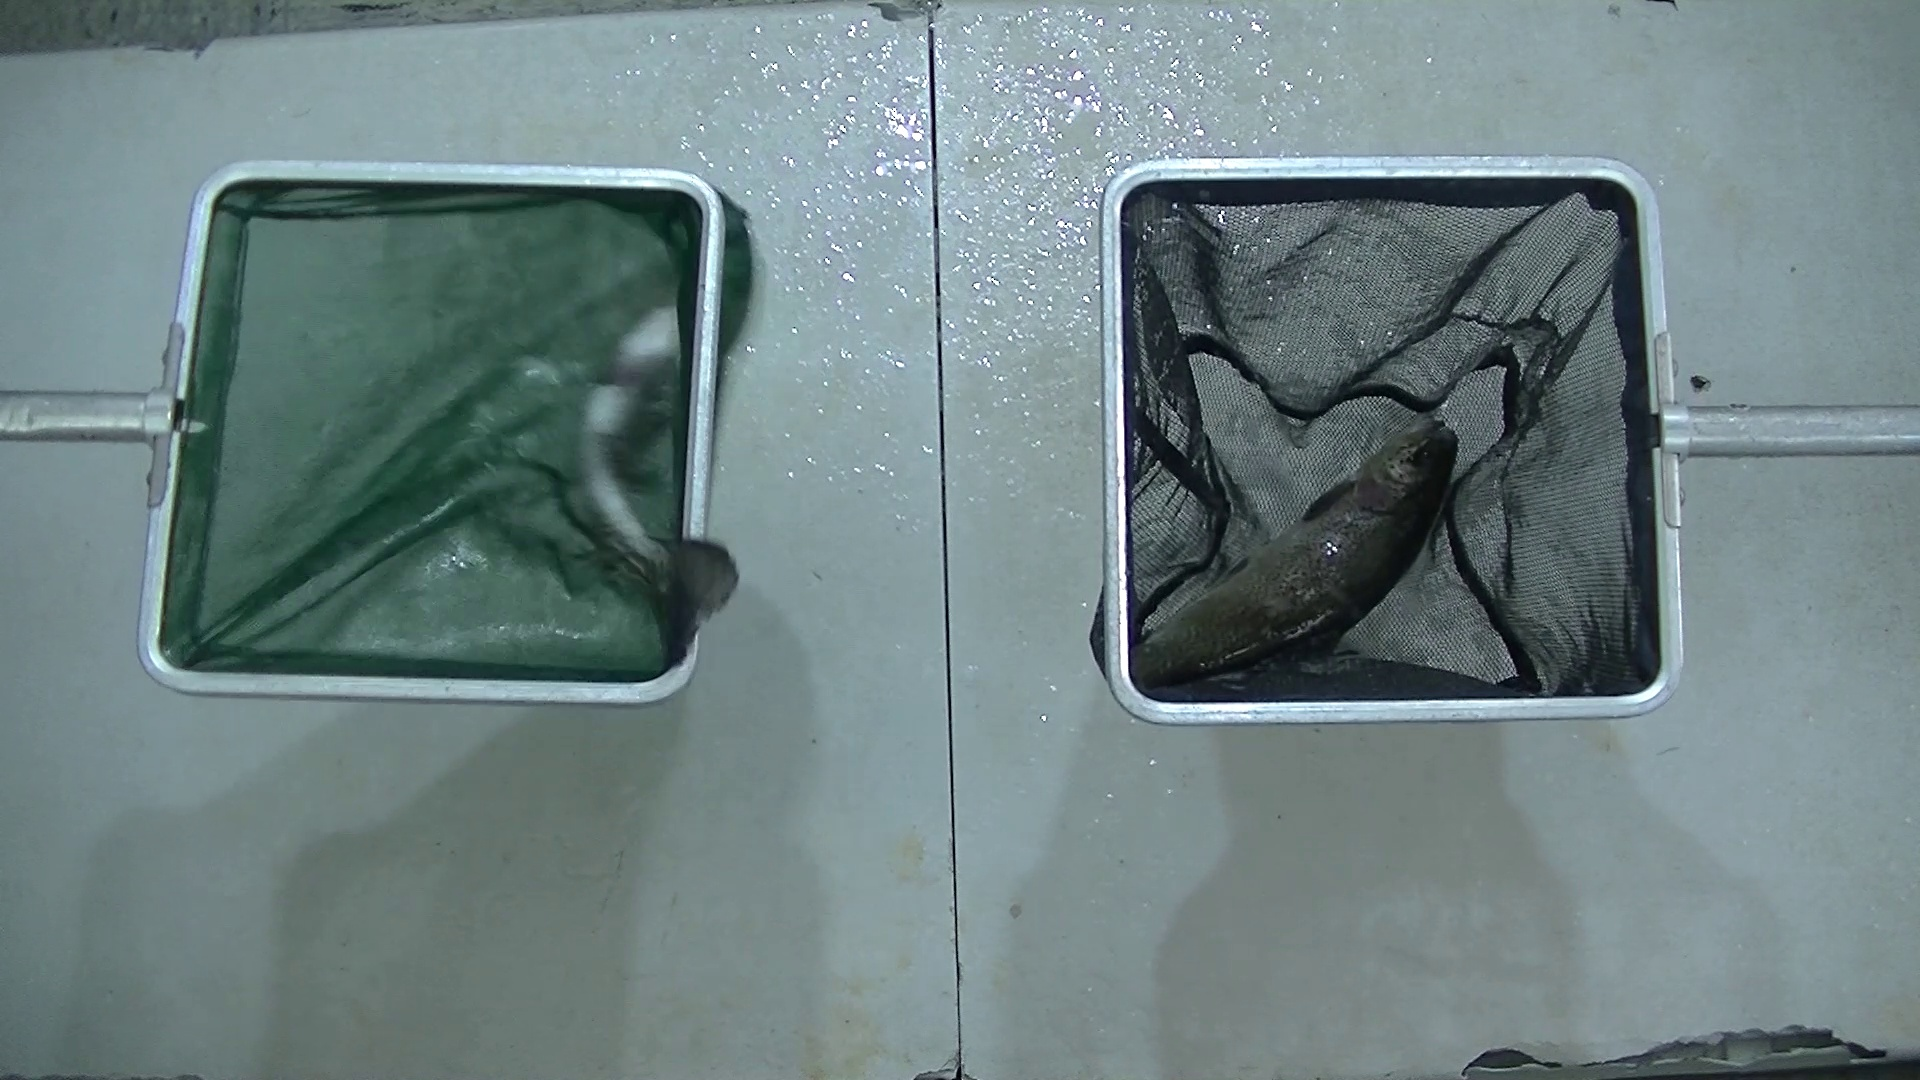
\includegraphics[width=0.7\textwidth]{images/6/6.3/RedNegra.jpg}
    \caption{Fotograma de ejemplo en videos con red negra}
    \label{fig:RedNegra}
\end{figure}

Para solucionar este problema y como entrenamiento final, se decidió hacer un último aumento del conjunto de datos. Para esto se tomaron imágenes aleatorias de los videos \verb|23_NT_R2_J1_P1_P2|, 
\verb|23_NT_R3_J1_P1_P2| y \verb|23_NT_R3_J2_P1_P2|. En total el conjunto de datos fue aumentado hasta los 203 fotogramas.\newline
Esto sumado a expandir el entrenamiento hasta las 600 épocas, permitió crear un modelo entrenado muy robusto para todo tipo de iluminaciones, cambios de redes y de variaciones de fondo.



\clearpage

Para poder aprovechar los diferentes recursos del sistema, se trabajó con 3 formatos de redes neuronales en los que \texttt{YOLO} es capaz de trabajar:
\begin{itemize}
    \item \textbf{PyTorch}: formato muy estandarizado y con soporte muy amplio. Es capaz de trabajar en \acrshort{cpu}, \acrshort{gpu} e incluso en dispositivos especializados para multiplicaciones de matrices como 
    las \acrfullr{tpu}. Su principal problema es que no está optimizado realmente para funcionar en \acrshort{cpu}. Obteniendo muy malos tiempos por fotograma. Su uso ideal es sobre las \texttt{GPU} de \texttt{NVidia}, 
    aprovechando el uso de operaciones \texttt{CUDA} para hacer cálculos con matrices. 
    \item \textbf{ONNX}: plataforma de traducción abierta entre modelos, ofrece mucho mejor soporte a distintos \texttt{HardWare} y ofrece mejor rendimiento si se quiere inferir sobre \texttt{cpu}.
    \item \textbf{OpenVino}: plataforma propietaria de \texttt{Intel}, que optimiza redes neuronales para todo el \texttt{HardWare} de su marca. Las redes neuronales exportadas en este formato son capaces 
    de aprovechar operaciones \texttt{\acrfullr{simd}}, consiguiendo aprovechar \texttt{GPUs} de \texttt{Intel} y mejorar mucho el rendimiento.
\end{itemize}

En un ordenador con un \texttt{i7-8700} y una \texttt{GTX 1060 6GB} se han visto los resultados para cada modelo mostrados en la \autoref{DiferenciasFormatos}.

\begin{table}[H]
    \begin{center} {
    \begin{tabular}{lc}
    \hline
     & \multicolumn{1}{c}{tiempo (ms) por fotograma}\\
    \hline
    \raisebox{0ex}{PyTorch-CPU} & 60 \\[0ex]
    \raisebox{0ex}{PyTorch-CUDA} & 10 \\[0ex]
    \raisebox{0ex}{ONNX} & 40 \\[0ex]
    \raisebox{0ex}{OpenVino} & 13 \\[0ex]
    \hline
    \end{tabular} }
    \end{center}
    \caption{Diferencia de tiempo de inferencia por formato de modelo de \texttt{YOLO}}
    \label{DiferenciasFormatos}
\end{table}

Más tarde en el documento se verá la integración de estos diferentes modelos en la aplicación y en el uso dependiendo del \texttt{HardWare} del usuario.

\clearpage

\subsection{Análisis del número de movimientos en el video}



Se buscó desarrollar un sistema secuencial como el representado en la \autoref{fig:IdeaSistemaBasico}, donde se utiliza \texttt{YOLO} para procesar los videos y detectar en cada fotograma 
una \texttt{Bounding Box} de la trucha. Posteriormente estos datos son procesados y, a través de la aplicación de un algoritmo, se detecta el número de movimientos que han ocurrido y cuando han sucedido.

\begin{figure}[H]
    \centering
    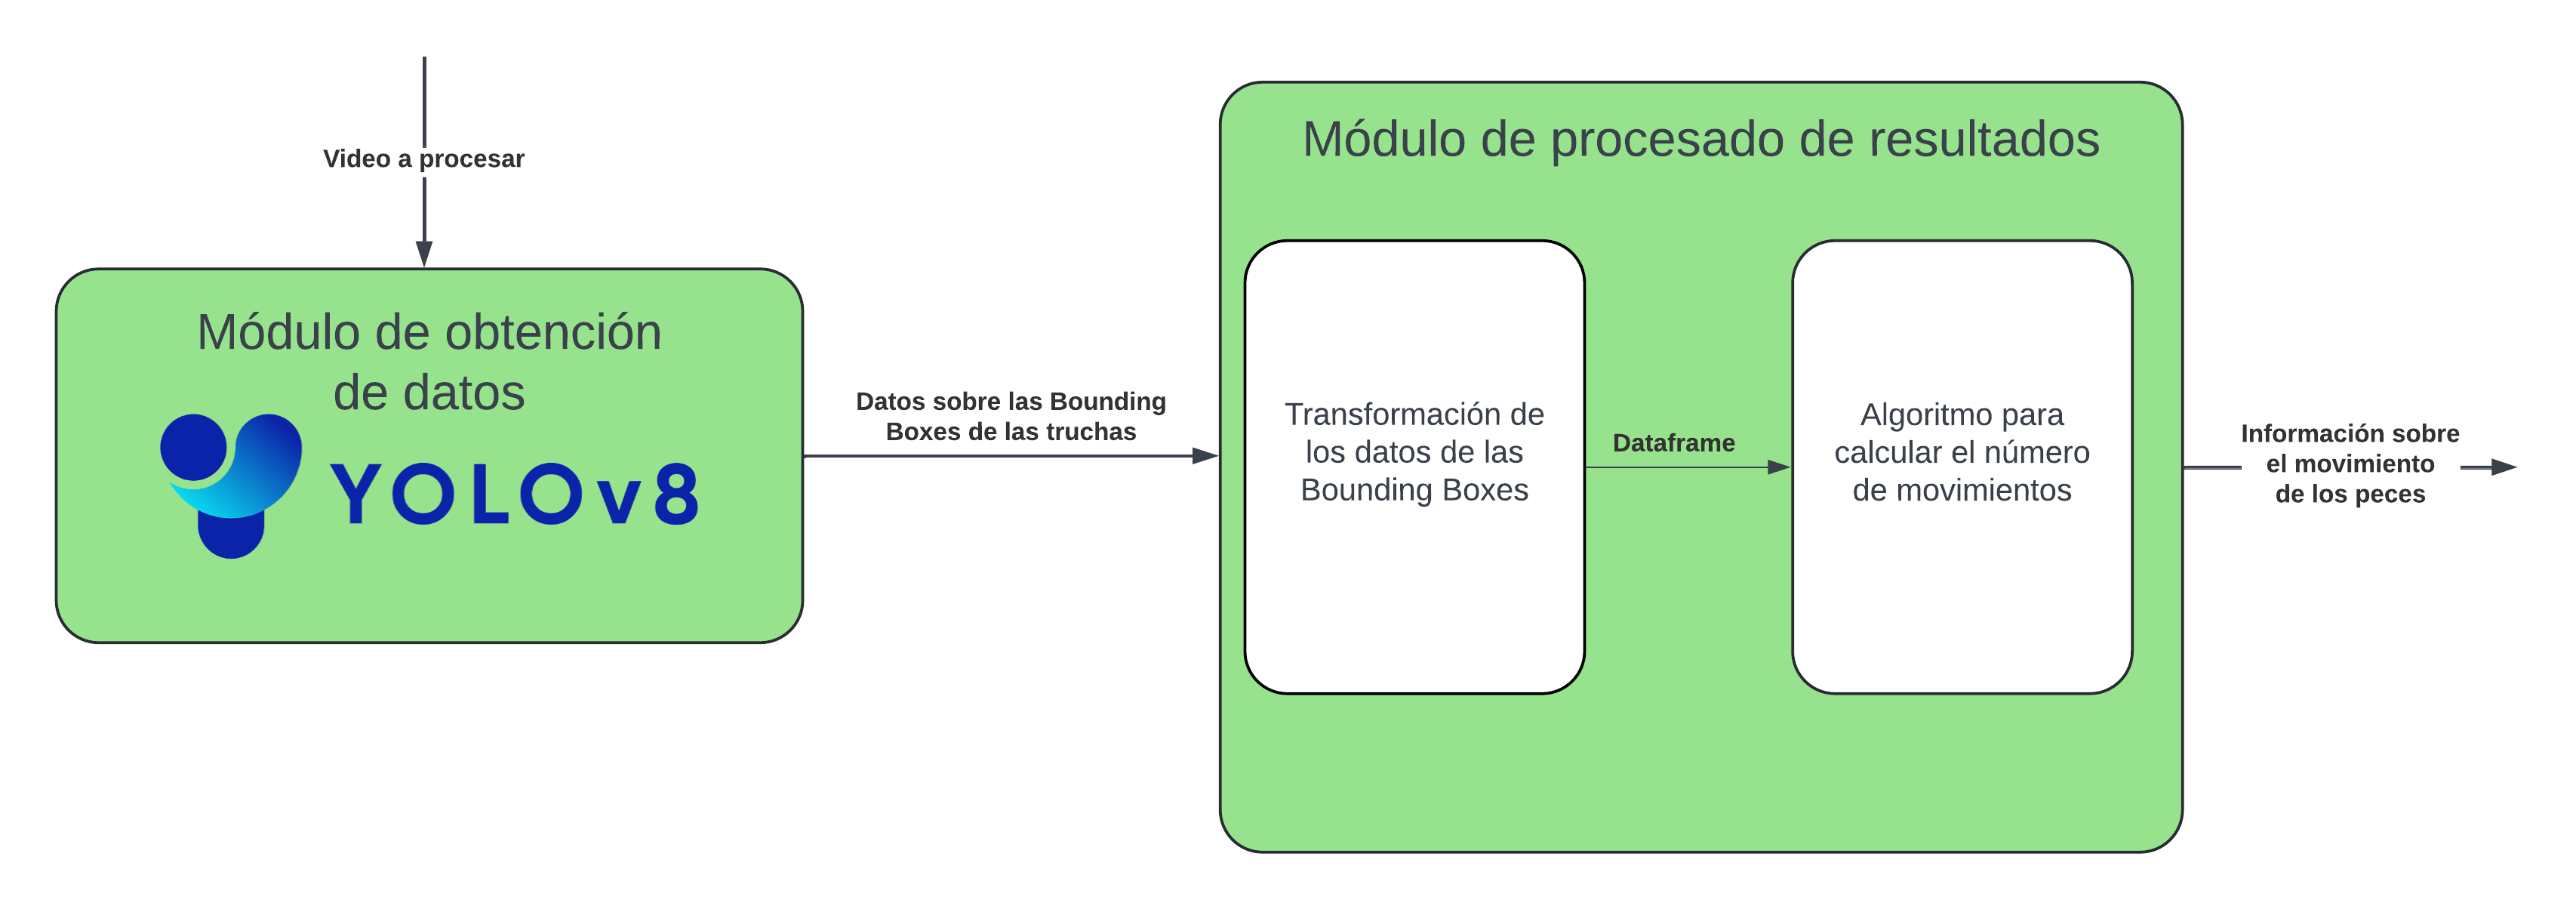
\includegraphics[width=\textwidth]{images/6/6.3/DiagramaStandAlone.png}
    \caption{Diagrama del primer sistema secuencial desarrollado}
    \label{fig:IdeaSistemaBasico}
\end{figure}

Para plantear el procesamiento, primero se deben entender que datos es capaz de devolver un modelo \texttt{YOLO}, su formato y seleccionar los mas relevantes. Esto depende en gran medida del tipo de 
modelo que se esté usando.

\subsubsection{Obtención del número de truchas en el video}

Los modelos de detección habitual de \texttt{YOLO} devuelven un objeto \texttt{ultralytics.engine.results}, cuyo contenido relevante para este trabajo ha sido:

\begin{itemize}
    \item \textbf{Boxes}: objeto con información sobre los elementos detectados, tamaño, posición y confianza de clasificación.
    \item \textbf{OBB}: en este caso es \texttt{None} por que no se realiza este tipo de tarea.
    \item \textbf{Imagen original}: objeto que contiene la imagen original de ese fotograma.
    \item \textbf{Tamaño de la imagen}: diccionario de dos elementos con el tamaño de la imagen de tipo \texttt{(ancho, altura)} expresado en píxeles.
\end{itemize}

Sin embargo, los modelos que se basan en detectar \texttt{Bounding Boxes} orientadas devuelven:

\begin{itemize}
    \item \textbf{Boxes}: en este caso \texttt{None}
    \item \textbf{OBB}: objeto con la información sobre las detecciones, igual que \texttt{Boxes} en contenido pero estructurado de forma diferente.
    \item \textbf{Imagen original}.
    \item \textbf{Tamaño de la imagen}.
\end{itemize}

\clearpage

De los elementos anteriores que contienen la información de las \texttt{Bounding Boxes}, se deciden utilizar ciertos elementos respectivamente:
\begin{itemize}
    \item \textbf{Boxes}: Este objeto contiene un elemento llamado \texttt{xywh} conteniendo la posición \texttt{x} e \texttt{y} del centro de cada \texttt{Bounding Boxes} en la imagen respecto a la esquina 
    superior izquierda. Además contiene el ancho \texttt{w} y el alto \texttt{h} de cada una. Es de tipo \texttt{Tensor} internamente.
    \item \textbf{OBB}: Este objeto contiene un elemento llamado \texttt{xywhr} igual que el elemento anterior, pero al ser cajas orientadas, se añade un elemento extra que representa la rotación de la \texttt{Bounding Box}.
\end{itemize}

Una vez se obtienen todos estos elementos de un video, es necesario saber el pez al que pertenece para \texttt{Bounding Box} detectada. Esto es importante, ya que estos sistemas pueden detectar varias instancias de un objeto en la 
misma posición de forma superpuesta. Un ejemplo de esto se ve en la \autoref{fig:Superposicion}. En este caso es esperable obtener 1 datos por fotograma, por lo tanto se decide la mejor \texttt{Bounding Box}.

\begin{figure}[H]
    \centering
    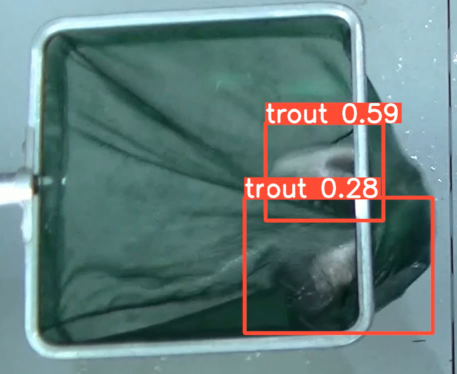
\includegraphics[width=0.5\textwidth]{images/6/6.3/Superposicion.png}
    \caption{Presencia de varias \texttt{Bounding Boxes} superpuestas para una trucha en el experimento}
    \label{fig:Superposicion}
\end{figure}

Para saber cuantos peces aparecían en el video, se utilizó la media de la posición \texttt{x} de las primeras 50 muestras para analizar el punto medio de la imagen entre los datos. 
Posteriormente se calcula la desviación de las muestras para analizar si la desviación es mayor a un límite según la resolución del video. Este sistema permite saber si hay 1 o 2 truchas en el experimento, 
añadiendo flexibilidad al sistema.

Posterior a esto, se realiza una transformación de datos para construir un objeto \texttt{DataFrame} de la librería \texttt{Pandas}, usada en la ciencia de datos por su capacidad de manejar muchos datos de forma 
extremadamente rápida, ya que internamente utiliza el lenguaje de programación \texttt{C}. \newline
Para cada fotograma, se selecciona la \texttt{Bounding Box} que ha tenido mayor confianza por la red para cada zona en la que existe una trucha. Cada índice de este \texttt{dataframe} representa el fotograma y 
el contenido de cada columna será un diccionario de \texttt{Python} con la información relevante. Esto se puede ver en la \autoref{fig:DatosEstructurados}.
\begin{figure}[H]
    \centering
    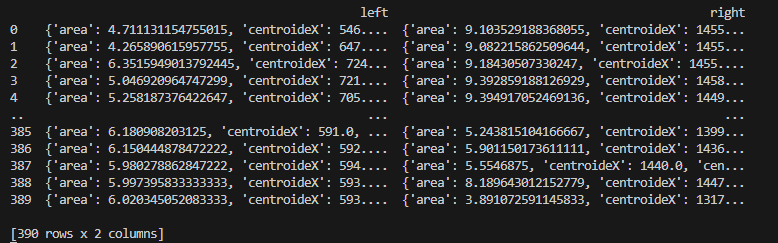
\includegraphics[width=0.9\textwidth]{images/6/6.3/DatosEstructurados.png}
    \caption{Datos estructurados procesados por fotograma y por trucha para las \texttt{Bounding Boxes}}
    \label{fig:DatosEstructurados}
\end{figure}

\clearpage

De forma más concreta, por cada trucha y por cada fotograma se guarda:
\begin{itemize}
    \item Área de la \texttt{Bounding Box} en porcentaje respecto a la resolución de la imagen.
    \item Posición \texttt{X} del centroide de la \texttt{Bounding Box}.
    \item Posición \texttt{Y} del centroide de la \texttt{Bounding Box}.
    \item Relación del ancho entre la altura de la \texttt{Bounding Box}.
    \item Ángulo de rotación (Si no es detección \acrshort{obb}, será 0).
    \item Valor del \texttt{Blur}: Se guarda la varianza del filtro laplaciano sobre la sección donde se encuentra la trucha. Esto es interesante porque un movimiento de una trucha implica una imagen más borrosa. A través 
    del filtro laplaciano podemos buscar bordes, y cuantos menos aparezcan en la imagen, menor será la varianza.
\end{itemize}

\subsubsection{Obtención de los movimientos de cada trucha}

El \texttt{DataFrame} con todos los datos se procesa de la siguiente manera:
\begin{enumerate}
    \item Para cada columna de trucha, se realiza un nuevo \texttt{DataFrame} que almacene en columnas separadas los valores de área, centroides, \texttt{blur}, etc. Esto es para no tratar con diccionarios.
    \item Se calcula el gradiente de la columna del área. Esto nos permite ver el cambio entre fotogramas de área y es uno de los puntos importantes a la hora de buscar movimientos.
    \item Se calcula el cambio absoluto de la posición del centroide de las \texttt{Bounding Boxes} entre fotogramas.
\end{enumerate}

Con el procesamiento de los datos realizados, se puede aplicar el algoritmo para buscar movimientos, que utiliza el siguiente pseudocodigo:
\begin{algorithm}
    \caption{Estimación de movimiento}
\begin{algorithmic}[1]
    \State $GradienteTotalSubconjunto \gets \texttt{suma de los gradientes del subconjunto}$
    \If{$gradienteTotalSubconjunto \geq -1 $} 
        \State $return -1$
    \ElsIf{$\texttt{todos los valores del gradiente del subconjunto} \geq -0.8$}
        \State $return -1$
    \ElsIf{$0.3 \leq \texttt{Todos los valores de la relacion x/y del subconjunto} \leq 2.7$}
        \If{$\texttt{El mayor área del subconjunto} \geq \texttt{mediana de los datos}\cdot0.9$}
            \State $return -1$
        \Else{$ $}
            \State $resultado \gets \texttt{Fotograma del subconjunto con menor varianza del Blur}$
            \State $return \texttt{  resultado}$
            \EndIf
    \Else{$ $}
        \State $return -1$
    \EndIf
\end{algorithmic}
\end{algorithm}\newline
Al algoritmo se le pasan todos los subconjuntos de fotogramas en los que el gradiente ha sido menor que 0, siendo necesario que sean subconjuntos mayores a 1 elemento y menores a 9. Esto ayuda a eliminar 
situaciones en las que la \texttt{Bounding Box} cambia mucho entre fotogramas sin ningún movimiento de la trucha. Posteriormente, dentro del algoritmo se verifican los datos para eliminar situaciones 
que pueden ser errores o pueden no ser representativas de un movimiento.

\clearpage
